%-  LaTeX source file

%-  overview.tex ~~
%
%   This is the second section of the paper.
%
%                                               ~~ (c) SRW, 20 Sep 2018
%                                               ~~ last updated 23 Sep 2018

PanDA is a Workload Management System (WMS) [marco2009glite] designed to
support the execution of distributed workloads and workflows via pilots
[turilli2017comprehensive]. Pilot-capable WMS enable high throughput of tasks
execution via multi-level scheduling while supporting interoperability across
multiple sites. This is particularly relevant for LHC experiments, where
millions of tasks are executed across multiple sites every month, analyzing
and producing petabytes of data. The design of PanDA WMS started in 2005 to
support ATLAS.

% ---------------------------------------------------------------------------
\subsection{Design}
\label{subsec:design}

PanDA's application model assumes tasks grouped into workloads and workflows.
Tasks represent a set of homogeneous operations performed on datasets stored
in one or more input files. Tasks are decomposed into jobs, where each job
consists of the task's operations performed on a partition of the task's data
set. PanDA's usage model assumes multitenancy of resources and at least two
types of HEP users: individual researchers and groups executing so called
``production'' workflows. Production workflows is a set of transformations of
collected and simulated data into formats which are used for user analysis.

PanDA's security model is based on separation between authentication,
authorization and accounting for both single users and group of users. Both
authentication and authorization are based on digital certificates and on the
virtual organization abstraction [foster2001anatomy]. Currently, PanDA's
execution model is based on four main abstractions: task, job, queue, and
pilot. Both tasks and jobs are assumed to have attributes and states and to
be queued into a global queue for execution. Prioritization and binding of
jobs are assumed to depend on the attributes of each job. Pilot is used to
indicate the abstraction of resource capabilities. Each job is bound to one
pilot and executed at the site where the pilot has been instantiated.

In PanDA's data model, each datum refers to the recorded or simulated
measurement of a physical process. Data can be packaged into files or other
containers. As with jobs, data have both attributes and states, and some of
the attributes are shared between events and jobs. Raw, reconstruction, and
simulation data are all assumed to be distributed across multiple storage
facilities and managed by the ATLAS Distributed Data Management (DDM)
[garonne2012atlas]. When necessary, input files required by each job are
assumed to be replicated over the network, both for input and output data.
PanDA's design supports provenance and traceability for both jobs and data.
Attributes enable provenance by linking jobs and data items, providing
information like ownership or project affiliation. States enable traceability
by providing information about the stage of the execution in which each job
or data file is or has been.

% ---------------------------------------------------------------------------
\subsection{Implementation and Execution}
\label{subsec:implementation}

The implementation of PanDA WMS consists of several interconnected
subsystems, most of them built from off-the-shelf and Open Source components.
Subsystems communicate via messaging using HTTP and dedicated APIs, and each
subsystem is implemented by one or more modules. Databases are used to store
eventful entities like tasks, jobs, and input/output data and to store
information about sites, resources, logs, and accounting.

Currently, PanDA's architecture has five main subsystems: PanDA Server
[maeno2011overview], AutoPyFactory [caballero2012autopyfactory], PanDA Pilot
[nilsson2011atlas], JEDI [borodin2015scaling], and PanDA Monitoring
[klimentov2011atlas]. PanDA uses ATLAS Grid Information system (AGIS)
[1742-6596-513-3-032001] to obtain information about distributed resources.

Other subsystems are used by some of ATLAS workflows (e.g., ATLAS Event
Service [calafiura2015atlas]), but their discussion is omitted here because
they are irrelevant to understanding how PanDA has been ported to
supercomputers. For a full list of subsystems, see Ref. [panda-wiki\_url].
Figure \ref{fig:architecture} shows a diagrammatic representation of PanDA's
main subsystems, highlighting the execution process of tasks while omitting
monitoring details to improve readability. During first LHC data taking
period (LHC Run 1), PanDA required users to perform a static conversion
between tasks and jobs; tasks were described as a set of jobs and then
submitted to the PanDA Server. This introduced inefficiency both with
usability and resource utilization. Ideally, users should conceive analyses
in terms of one or more potentially related tasks, while the workload manager
(i.e., PanDA) should partition tasks into jobs, depending on execution
constraints. Further, the static partitioning of tasks into jobs does not
take into account the heterogeneous and dynamic nature of the resources on
which each job will be executed, introducing inefficiencies.

% For two-column wide figures use
\begin{figure*}
% Use the relevant command to insert your figure file.
% For example, with the graphicx package use
  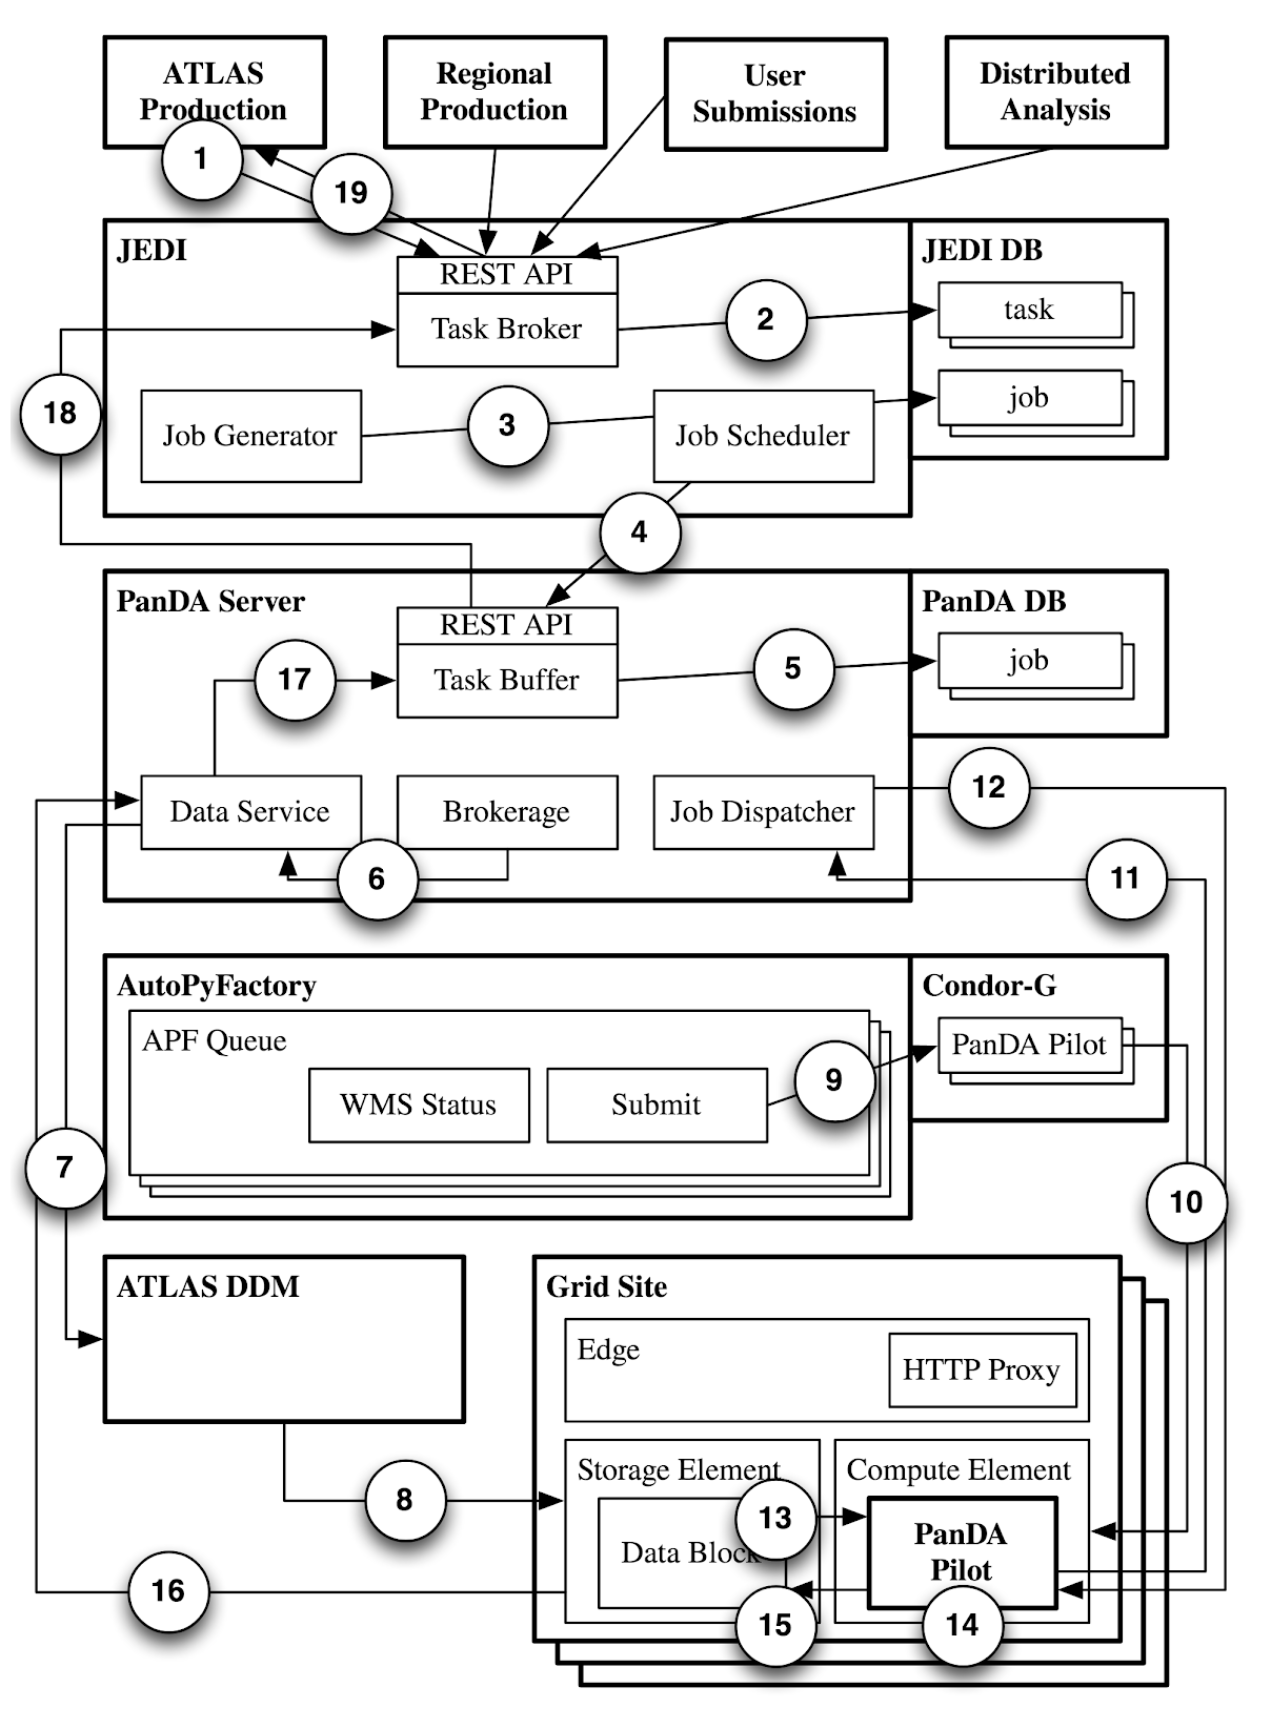
\includegraphics[width=0.75\textwidth]{images/Figure_1_placeholder.png}
% figure caption is below the figure
\caption{PanDA WMS architecture. Numbers indicate the JEDI-based execution
process described in section \ref{subsec:implementation}. Several subsystems,
components, and architectural and communication details are abstracted to
improve clarity.}
\label{fig:architecture}
\end{figure*}

% OKAY, PROBLEM. I think the "Fig. 1:n" stuff in the next paragraph refers
% not to a new figure, but to specific numbered pieces of Figure 1. I'm going
% to link them all to the figure and hardcode the ":n" part but not the
% figure number.

Another problem of static job sizing is that PanDA instantiates pilots on
sites with different type of resources and different models of availability
of those resources. An optimal sizing of each job should take these
properties into account. For example, sites may offer cores with different
speeds, networking with different amounts of bandwidth, and resources with
different availabilities which may or may not be guaranteed for known amounts
of time. These resources could disappear at any point in time, as often
happens with opportunistic models of resource provision. JEDI system was
deployed to address these inefficiencies. Users submit task descriptions to
JEDI (Fig.~\ref{fig:architecture}:1), which stores them into a queue
implemented by a database (Fig.~\ref{fig:architecture}:2). Tasks are
partitioned into jobs of different sizes, depending on both static and
dynamic information about available resources
(Fig.~\ref{fig:architecture}:3). Jobs are bound to sites with resources that
best match jobs' requirements, and they are submitted to the PanDA Server for
execution (Fig.~\ref{fig:architecture}:4).

Once submitted to the PanDA Server, tasks are stored by the Task Buffer
component into a global queue implemented by a database
(Fig.~\ref{fig:architecture}:5). When jobs are submitted directly to the
PanDA Server, the Brokerage module is used to bind jobs to available sites,
depending on static information about the resources available for each site.
Jobs submitted by JEDI are already bound to sites, so no further brokerage is
needed.

Once jobs are bound to sites, the Brokerage module communicates to the Data
Service module about which datasets need to be made available to which sites
(Fig.~\ref{fig:architecture}:6). The Data Service communicates these
requirements to the ATLAS DDM (Fig.~\ref{fig:architecture}:7) which
replicates datasets at the required sites when needed
(Fig.~\ref{fig:architecture}:8).

Meanwhile, AutoPyFactory defines PanDA Pilots, submitting them to a Condor-G
agent (Fig.~\ref{fig:architecture}:9). Condor-G schedules these pilots
wrapped as jobs or virtual machines to the required sites
(Fig.~\ref{fig:architecture}:10).

When a PanDA Pilot becomes available, it requests a job to execute from the
Job Dispatcher module of the PanDA Server (Fig.~\ref{fig:architecture}:11).
The Job Dispatcher interrogates the Task Buffer module for a job which is
bound to the site of that pilot and ready to be executed. Task Buffer checks
the global queue (i.e., the PanDA database) and returns a job to the Job
Dispatcher if one is available. The Job Dispatcher dispatches that job to the
PanDA Pilot (Fig.~\ref{fig:architecture}:12).

Upon receiving a job, a PanDA Pilot starts a monitoring process and forks a
subprocess for the execution of the job's payload. Input data are transferred
from the stage-in location (Fig.~\ref{fig:architecture}:13) and the job's
payload is executed (Fig.~\ref{fig:architecture}:14). Once completed, output
is transferred to the staging-out location (Fig.~\ref{fig:architecture}:15).

The Data Service module of the PanDA Server tracks and collects the output
generated by each job (Fig.~\ref{fig:architecture}:16), updating jobs'
attributes via the Task Buffer module (Fig.~\ref{fig:architecture}:17). When
the output of all the jobs of a task are retrieved, it is made available to
the user via PanDA Server. When a task is submitted to JEDI, task is instead
marked as done (Fig.~\ref{fig:architecture}:18) and the result of its
execution is made available to the user by JEDI
(Fig.~\ref{fig:architecture}:19).

% ---------------------------------------------------------------------------
\subsection{Job-State Definitions in PanDA}
\label{subsec:jobstatedefs}

The lifecycle of the job in the PanDA system is splitted to the series of
consequently changing states. Each state literally coupled with the PanDA job
status used by the different algorithms and monitoring. Status reflect the
current step of the job processing since the job submitted to the system,
transferred to the particular resource and finally executed.

Job injected into the system by the JEDI in ATLAS or by the PanDA client in
general case is persist as so-called job parameters object and corresponds to
the ``Pending'' status. Job parameters are the object where job definition is
unsorted and all parameters are placed in a string. Sorting out parameters of
the job by dedicated DB fields job transferring into the ``Defined'' status.
On this stage the job is processed throw the brokerage algorithm and being
assigned to particular resource (PanDA queue) it is moved to ``Assigned''
status. Concurrently with that PanDA server checks availability of the input
data and needed SW at the resource. The job stays in the ``Waiting'' state
until data and the SW are ready and then it moved to the ``Activated''
status. Activated job is ready to be dispatched by its order to the next
corresponding pilot. Job dispatched and taken by the pilot is moved to the
``Sent'' status. Since this moment the handling of the job processing is
delegated to the pilot. Few next job states are corresponding represents the
steps of the job processing on the resource. Next ``Starting'' status means
that the pilot is starting the job on a worker node or local batch system.
The job running on a worker node marked as in ``Running'' status. Next states
progression is return to the handling by the server. When the job execution
is ended and output and log files are transferred then PanDA server either
pilot is responsible to register that files in the file catalog. At the same
time pilot return the server the final status of the job either it was
successful or the job failed. During this process the job stays in
``Holding'' status. PanDA server check the output files regularly by the cron
job and finally assign the final ``Finished'' or ``Failed'' status to the
job. Some additional statuses and two most important are ``Cancelled'' for
manually killed jobs or ``Closed'' - terminated by the system before
completing to be reassigned to another site.

% ---------------------------------------------------------------------------
\subsection{Brokerage Characterization}
\label{subsec:brokerage}

Resources (queues) presented in the database together with the wide set of
static parameters such as walltime, CPU cores, memory, disk space etc. Same
parameters can be provided within job definition to specify strict demands to
the resource where the job can be executed. Both resources (queues) and jobs
with parameters stored in the PanDA database.

Also PanDA server maintains in the DB the dynamic information for queues
about the number of defined, activated and running jobs and also the pilots
statistics - number of requests of different types like ``get job'' or
``update job status''.

PanDA Broker - key  component of the BigPanDA workflow automation - is an
intelligent module designed to prioritize and assign PanDA jobs (job passed
the brokerage transitioning from ``defined'' to the ``assigned'' state) to
available computing resources on the basis of job type, software
availability, input data and its locality, real-time job statistics,
available CPU and storage resources and etc. Users are able to specify
explicitly the resource while job submission or they can rely on automated
brokerage engine. Full power of the PanDA brokerage integrated with another
distributed computing and data management tools (internal and external with
respect to the PanDA) is actively used in ATLAS experiment. In this paper we
will present and will benchmark the basic brokerage functionality provided to
all users.

The basic brokerage algorithm works the following way. It takes the lists of
submitted jobs and available queues. Then each job is checked against each
queue by set of parameters if the queue meets the jobs static demands like
number of CPU core or the walltime. All queues passed the round are
proceeding to the short list where for each queue Broker calculates the
weight on the basis of current job statistics for given queue according to
the formula (1). Job finally assigning to the queue with bigger weight.
Weight calculation algorithm fo ATLAS is more complicated and taking into
account clouds default weights, network bandwidth, sharing policies etc.

The basic brokerage algorithm works the following way. Having the list of the
submitted jobs, each job is checked against available resources as shown in
SELECT{\textunderscore}CAND (Alg. ). Available resources presented as the set
of defined PanDA queues: res = queue$_1$, \ldots, queue$_n$. For each queue
in the set (3) we checking if it's satisfying the parameters of job (4).
Successfully passed queues are concatenating to the list of candidate-queues
(5).

SATISFY{\textunderscore}JOB function (Alg. ) is used to check if the queue
attributes can scope job parameters. Set of the job parameters defined as
par$_1$, \ldots, par$_m$ represents the software/hardware demands to the
resource like CPU core count, walltime, SW releases etc. Each of these
parameters can be mapped to the set of queue attributes defined as atr$_1$,
\ldots, atr$_n$, where $n \geq m$. So for each job parameter (2) we check if
it can be satisfied with the corresponding queue attribute (3). Finally queue
passes the test if it copes all the jobs parameters (5).

The procedure SATISFY{\textunderscore}REQ (Alg. ) is responsible to testing
if the value of the job parameter is in the set of allowed values val$_1$,
\ldots, val$_k$ of the queue attribute (2).

%-  NOTE: I think there are indenting mistakes present in the original
%   writing, because things just honestly don't look right to me, but right
%   now, I'm just typesetting what I see in Google Docs.


% I have already included the package required by this. Just put the code
% list.py file (or whatever other name you want to use.)

\lstinputlisting[language=Python, 
         label={lst:list.py}, 
         caption={Caption}]{list.py}

\begin{tabbing}
\hspace{0.5in}\=
     Require: par; atr = (val$_1$, \ldots, val$_k$) \\
  \> Ensure: True or False \\
  \> 1: \hspace{1em}\= procedure SATISFY{\textunderscore}REQ(par, atr) \\
  \> 2:             \> \hspace{1em}\= if par.value in atr then: \\
  \> 3:             \>             \> return True \\
  \> 4:             \>             \> \hspace{0.1in} return False
\end{tabbing}

\begin{tabbing}
\hspace{0.5in}\=
     Require: job = \{par$_1$, \ldots, par$_m$\}; queue = \{atr$_1$, \ldots, atr$_n$\} \\
  \> Ensure: True or False \\
  \> 1: \hspace{1em}\= procedure SATISFY{\textunderscore}JOB(queue, job) \\
  \> 2:             \> \hspace{1em}\= for all par in job do: \\
  \> 3:             \>             \> if SATISFY{\textunderscore}REQ(par, atr)%
= False then \\
  \> 4:             \>             \> \hspace{2em} return False \\
  \> 5:             \>             \> \hspace{1em} return True
\end{tabbing}

\begin{tabbing}
\hspace{0.5in}\=
     Require: job; res = (queue$_1$, \ldots, queue$_n$) \\
  \> Ensure: cand \\
  \> 1: \hspace{1em}\= procedure SELECT{\textunderscore}CAND(job, res) \\
  \> 2:             \> \hspace{1em}\= cand $\leftarrow$ NONE \\
  \> 3:             \> \hspace{1em}\= for all queue in res do: \\
  \> 4:             \>             \> if SATISFY{\textunderscore}JOB(queue,%
job) = True then \\
  \> 5:             \>             \> \hspace{1em} cand $\cup$ queue \\
  \> 6:             \>             \> return True
\end{tabbing}

As it was shown SELECT{\textunderscore}CAND procedure provides generates the
short list of the candidates queues. SELECT{\textunderscore}QUEUE (Alg. )
taking the short list of the candidate-queues as the set queue$_1$, \ldots,
queue$_n$. For each queue (4) Broker calculates the weight (5) on the basis of
current job statistics for given queue according to the formula (1). Job
finally assigning to the queue with bigger weight (6-7). Weight calculation
algorithm fo ATLAS is more complicated and taking into account clouds default
weights, network bandwidth, sharing policies etc

\begin{tabbing}
\hspace{0.5in}\=
     Require: cand = (queue$_1$, \ldots, queue$_n$) \\
  \> Ensure: res{\textunderscore}queue \\
  \> 1: \hspace{1em}\= procedure SELECT{\textunderscore}QUEUE(cand) \\
  \> 2:             \> \hspace{1em}\= res{\textunderscore}queue $\leftarrow$%
queue$_1$ \\
  \> 3:             \>             \> \hspace{0.1in} max{\textunderscore}%
weight $\leftarrow 0$ \\
  \> 4:             \> \hspace{1em}\= for all queue in cand do: \\
  \> 5:             \>             \> queue.weight $\leftarrow$ %
WEIGHT{\textunderscore}CALC(queue) \\
  \> 6:             \>             \> \hspace{1em} if queue.weight $>$ %
max{\textunderscore}weight then \\
  \> 7:             \>             \> \hspace{2em} res{\textunderscore}queue%
$\leftarrow$ queue \\
  \> 8:             \>             \> \hspace{0.5em} return %
res{\textunderscore}queue
\end{tabbing}

\begin{equation}
  \begin{aligned}
    & manyAssigned = \max(1, \min(2, \frac{assigned}{activated})), \\
    & weight = \frac{running + 1}{(activated + assigned + sharing + defined +
        10) * manyAssigned}
  \end{aligned}
\end{equation}

Brokerage time in general can be estimated as (2). Basically it's time the job
transits from ``defined'' to assigned state.  

\begin{equation}
    T = \sum_{i = 1}^{Q} \sum_{j = 1}^{J} T_{ij}
\end{equation}

In formula (2) $Q$ is the number of available queues, $J$ is the number of
concurrently  submitted jobs and $T_{ij}$ is the time to process job $j$ for
queue $i$. The processing time includes the check if queue meet demands of the
job. Then for successfully selected queues the weight is calculating and job
assigning for the queue with bigger weight. Hence the time $T$ can be presented as sum (3).

\begin{equation}
T = t_1 + t_2 + t3_3 + C
\end{equation}

In formula 3, $t_1$ is the time to make checks if queue meet demands of the
job, $t_2$ is the time for weight calculation and finally $t_3$ is the time
spent to assign job to the resulted queue. 

Under the assumption that all jobs can run on the same average number of queues
$N$ then we can transform equation as (4).

\begin{equation}
T = J * \left ( \sum_{i = 1}^{Q - N} t1_j + \sum_{j = 1}^{N} (tmax + t2_j) + t3 \right) + C, t1 < tmax
\end{equation}

Here N is the average number of queues which met all demands of each job.  As shown in the SATISFY{\textunderscore}JOB algorithm the function returns FALSE as soon as the first discrepancy in the job parameter and queue attributes is met. Hence for for all other Q-N queues the time to make checks  t1 will be less than tmax.

Here N is the average number of queues which met all demands of each job. As shown in the SATISFY{\textunderscore}JOB algorithm the function returns False as
soon as the first discrepancy in the job parameter and queue attributes is met.
Hence for for all other Q-N queues the time to make checks t1 will be less than tmax.

Again taking assumption that the times for different queues are equal we can
streamline the equation like (5)

\begin{equation}
  \begin{aligned}
    T =& J * \left(( Q - N) * t1 + N * (tmax + t2) + t3 \right) + C \\
     =& J * \left(Q * t1 + N * (tmax - t1 + t2) + t3 \right) + C,
        \text{where}~(tmax - t1) > 0
  \end{aligned}
\end{equation}

In order to estimate dependency of brokerage time from the number of
concurrently submitted jobs we deployed a dedicated test instance of PanDA
server at ORNL. PanDA was configured to use ten testing queues. Two of the
queus was configured to provide 8 CPU cores and eight remaining queues provide
2 cores. All other parameters are configured equal for all queues.

Job submission client was configured to generate and send to the server the
lists of equal jobs where each job demands 4 CPU cores. PanDA testing-instance
was adjusted to simulate the brokerage two queues will be selected as meeting
the criteria of cores number. Then due to simulation of job statistics on that
selected queues the jobs will be assigned to the queue with bigger weight.
Brokerage time dependency on number of concurrently submitted jobs is shown in
figure.

% For two-column wide figures use
\begin{figure*}
% Use the relevant command to insert your figure file.
% For example, with the graphicx package use
  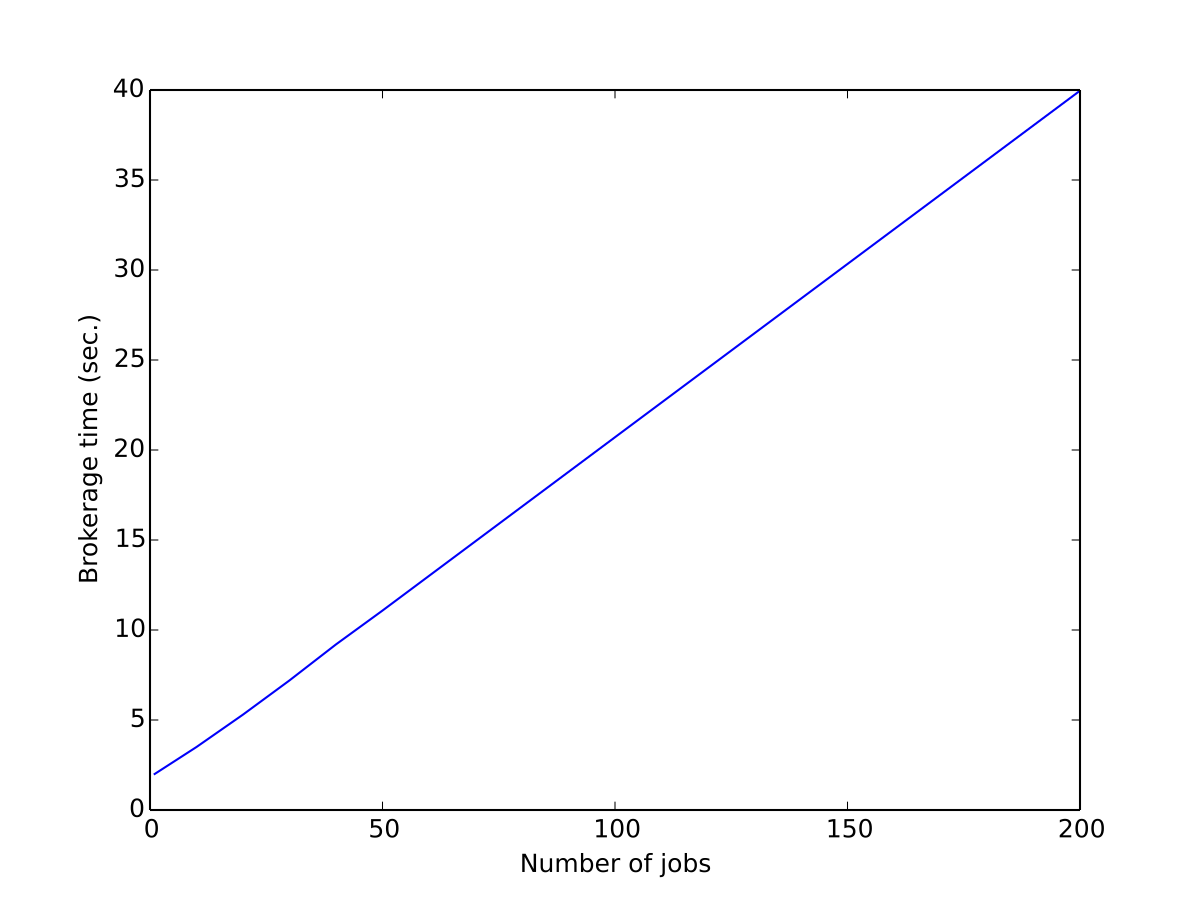
\includegraphics[width=0.75\textwidth]{images/Fig2.png}
% figure caption is below the figure
\caption{Brokerage time dependency on number of concurrently submitted jobs}
\label{fig:brokeragescaling}
\end{figure*}

For this experiment we measured the time for a jobs to transit from the
``Defined'' status to the ``Activated''. As in the test environment the JEDI
system wasn't used and injection of the jobs was done using the simple python
client interaction with PanDA REST API the first stated of the job indicated in
PanDA is ``Defined'' and corresponds to the creation time. Also during this
measurements we used no-input jobs. Hence the status of the jobs progressed to
the ``Activated'' immediately after ``Defined''. In general the time to check
input files can be considered as constant for the constant number of input
files. So omitting the ``Assigned'' state in this testing environment is
acceptable. 



%-  vim:set syntax=tex:
